\subsection{dOPT}
\label{algo:dopt}

\emph{dOPT} (Distributed Operational Transformation) is the first operational transformation algorithm developed by {Ellis and Gibbs}\cite{ellis} in 1989. It was soon discovered that in some situations the document replicas did not converge. This situation is known as the \emph{dOPT} puzzle.

The algorithm fails in cases where there is more than one concurrent operation from a user (see figure \ref{fig:doptpuzzle}). Given operation $O_{a}$ from site $a$ and operations $O_{b_{1}}$ and $O_{b_{2}}$ from site $b$, where $O_{a} \parallel O_{b_{1}}$, $O_{a} \parallel O_{b_{2}}$ and $O_{b_{1}} \rightarrow O_{b_{2}}$, \emph{dOPT} incorrectly applies inclusion transformation against $O_{b_{1}}$ and $O_{b_{2}}$ in sequence against $O_{a}$ at site $a$. Note however that $O_{b_{2}}$ is not context-equivalent with $O_{a}$ and therefore $IT(O_{a},O_{b_{2}})$ violates the precondition of inclusion transformation.

\begin{figure}[H]
 \centering
 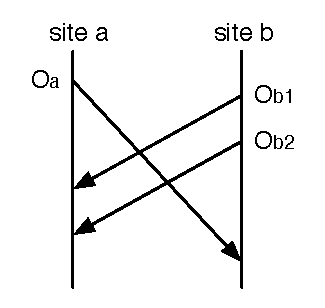
\includegraphics[width=1.94in,height=1.83in]{../../images/dopt_puzzle.eps}
 \caption{dOPT puzzle}
 \label{fig:doptpuzzle}
\end{figure}

Cormack\cite{cormack95a} detected this case and proposed a new algorithm (see \ref{algo:ccu}) that is only suitable for two sites connected by a point-to-point communication channel. He stated that there does not appear to be a simple and efficient correction to \emph{dOPT} that maintains its suitability for broadcast operations.

However Cormack showed in \cite{cormack95b} that using several point-to-point communication channels forming a tree it is possible to derive a consistent solution for an arbitrary number of sites (see also \ref{algo:netedit}).

\subsubsection{Properties}
\begin{itemize}
 \item algorithm is incorrect
 \item uses state vectors to maintain causal ordering
 \item uses linear history buffer (called request log)
 \item architecture: replicated, multicast
\end{itemize}
